% !TEX root = ../Rulebook.tex
\section{Test Specification Summary}
\renewcommand{\arraystretch}{1.1}
\newcommand{\R}[2]{
	\begin{turn}{90}
		\begin{minipage}[][1em][c]{#2}
		#1
	  \end{minipage}
	\end{turn}
}
\newcommand{\cir}[1]{\hspace{0.5em}\unitlength1ex\begin{picture}(2.8,2.8)%
\put(0.75,0.75){\circle{2.8}}\put(0.75,0.75){\makebox(0,0){#1}}\end{picture}}
\newcommand{\Y}{\tiny \CIRCLE}
\newcolumntype{P}[1]{>{\centering\arraybackslash}p{#1}}

\definecolor{headlineColor}{rgb}{.7,.7,.7}
\definecolor{sectionColor}{rgb}{.7,.1,.1}

\newcommand{\C}{\cellcolor{sectionColor}}
%\begin{landscape}
%\begin{table}[h!]
% \centering
% \begin{tabular}{|l|l|l*{11}{|P{1cm}}|}
%   \hhline{~~~--------}
%   \multicolumn{3}{l|}{ }                   &  \multicolumn{8}{c|}{Instances}                        \\
%   \hhline{~~~--------}
%   \multicolumn{3}{l|}{ }                   &\cir{1}&\cir{2}&\cir{3}&\cir{4}&\cir{5}&\cir{6}&\cir{7} \\
%   \multicolumn{3}{r|}{ }                   & BMT   & BTT1  & BTT2  &  BTT3 &  PPT  &  RTT  & Final  \\
%   \hhline{~~~--------} \hline
%   \multirow{5}{0.5cm}{\R{\centering Objects}{3.0cm}}
%   & \RCAW \&  RoCKIn            & atwork-commander   & 5     & 5     & 6     & 6     & 3      & 3     & 10    \\ \hhline{~----------}
%   & Decoy                       & TC   &       & 3     & 3     & 3     &        & 3     & 5     \\ \hhline{~----------}
%	 & Position                    &          & Ref   & Ref   & Ref   & Ref   & Team   & Ref   & Ref   \\ \hhline{~----------}
%	 & Rotation                    &          & Team  & Ref   & Ref   & Ref   & Team   & Team  & Ref   \\ \hhline{~----------}
%	 & Orientation                 &          & Team  & Team  & Team  & Ref   & Team   & Team  & Ref   \\ \hline
%   \multirow{6}{0.5cm}{\R{\centering Service area}{3.5cm}}
%   & Estimated Active            & atwork-commander   & 2     & 3     & 4     & 5     & 2      & 1     & 8     \\ \hline
%   & Table height                & atwork-commander   &       &       & 0 cm  &       &        &       &  0 cm \\
%   &                             &          &       &       & 5 cm  &       &        &       &  5 cm \\
%   &                             &          & 10 cm & 10 cm & 10 cm & 10 cm &  10 cm & 10 cm & 10 cm \\
%   &                             &          &       &       & 15 cm &       &        &       & 15 cm \\ \hhline{~----------}
%	 & Arbitrary surface           & TC   &       & 1     & 2     & 2     &        &       & 3     \\ \hline
%	 \multirow{3}{0.5cm}{\R{\centering Arena }{1.5cm}}
%	 & Physical Obstacles          & TC  &       &       & 2     & 2     &        &       & 2     \\ \hhline{~----------}
%	 & Virtual Obstacles           & TC  &       & 2     &       & 1     &        &       & 2     \\ \hhline{~----------}
%   &                             &          &       &       &       &       &        &       &       \\ \hhline{-----------}
%   \multirow{3}{0.5cm}{\R{\centering Grasping }{1.64cm}}
%   & Shelf unit                  & atwork-commander   &       &       &       & 2     &        &       & 2     \\ \hhline{~----------}
%	 & Rotating table          & Referee  &       &       &       &       &        & 3     & 1     \\ \hhline{~----------}
%   & Rotating direction          &          &       &       &       &       &        & Team  & Ref   \\ \hline
%   \multirow{8}{0.5cm}{\R{\centering Placement}{2.5cm}}
%   & Preisicon placement table  & atwork-commander   &       &       &       &       & 3      &       & 1     \\ \hhline{~----------}
%   & Shelf unit                  & atwork-commander   &       &       &       & 1     &        &       & 1     \\ \hhline{~----------}
%   & Red container               & atwork-commander   &       &       &       & 2     &        &       & 2     \\ \hhline{~----------}
%   & Blue container              & atwork-commander   &       &       &       & 2     &        &       & 2     \\ \hhline{~----------}
%   & Rotating turntable          & atwork-commander   &       &       & 1     &       &        &       &       \\ \hhline{~----------}
%   & Cavities Position           &    &       &       &       &       & Ref	   &       & Ref   \\ \hhline{~----------}
%   & Cavities Rotation	         &  &       &       &       &       & Ref    &       & Ref   \\ \hhline{~----------}
%   & Cavities Orientation	       &   &       &       &       &       & Team   &       & Team  \\ \hline \hline
%   \multicolumn{2}{|l|}{Duration}
%                                 & atwork-commander   & 5min  & 6min  & 10min & 10min & 4min   & 4min  & 13min \\
% 		\hline
% \end{tabular}
% \caption{Test specification in the instances of the \RCAW \YEAR competition.}
% \label{tab:Instances}
%\end{table}


\begin{figure}[h!]
	\centering
	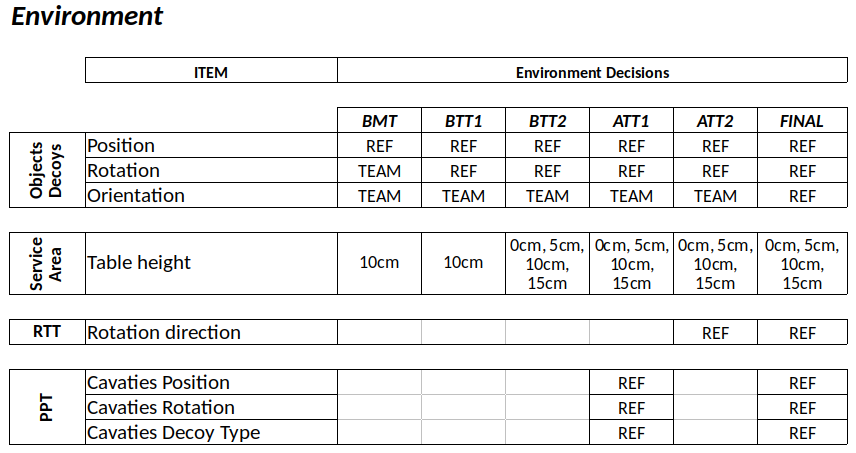
\includegraphics[width= 1.0\textwidth ]{./images/tabels/robocup_env.png}
	\caption{Test specification in the environment of the \RCAW \YEAR competition.}
	\label{fig:test_specifications_environment}
\end{figure}

\begin{figure}[h!]
	\centering
	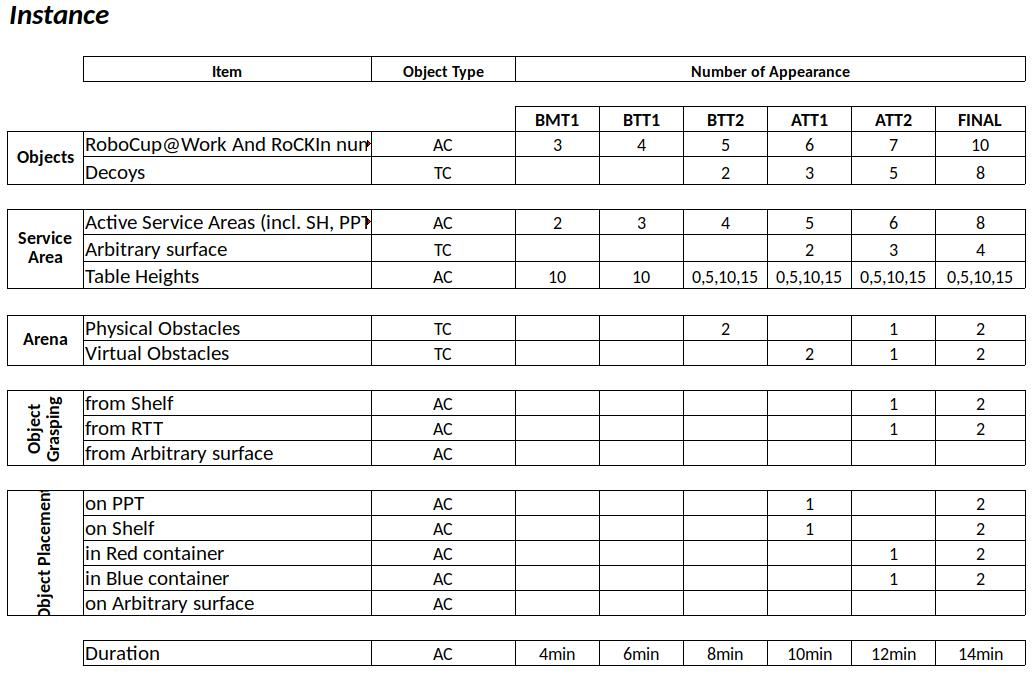
\includegraphics[width= 1.0\textwidth ]{./images/tabels/robocup_instance.jpg}
	\caption{Test specification in the instances of the \RCAW \YEAR competition.}
	\label{fig:test_specifications_instance}
\end{figure}
%\end{landscape}



